\nonstopmode
\documentclass{article}

% Language setting
% Replace `english' with e.g. `spanish' to change the document language
\usepackage[english]{babel}

% Set page size and margins
% Replace `letterpaper' with`a4paper' for UK/EU standard size
\usepackage[letterpaper,top=2cm,bottom=2cm,left=3cm,right=3cm,marginparwidth=1.75cm]{geometry}

% Useful packages
\usepackage{amsmath}
\usepackage{graphicx}
\usepackage[colorlinks=true, allcolors=blue]{hyperref}

\usepackage{pgfplots}
\usepackage{float}
\usepackage{amsfonts} 
\usepackage{array}
\usepackage{algorithm}
\usepackage{algpseudocode}
\usepgfplotslibrary{dateplot}
%\usepackage{url}
\usepackage{hyperref}

\usepackage{xparse}

\ExplSyntaxOn
\ior_new:N \g_hringriin_file_stream

\NewDocumentCommand{\ReadFile}{mm}
 {
  \hringriin_read_file:nn { #1 } { #2 }
  \cs_new:Npn #1 ##1
   {
    \str_if_eq:nnTF { ##1 } { * }
      { \seq_count:c { g_hringriin_file_ \cs_to_str:N #1 _seq } }
      { \seq_item:cn { g_hringriin_file_ \cs_to_str:N #1 _seq } { ##1 } }
   }
 }

\cs_new_protected:Nn \hringriin_read_file:nn
 {
  \ior_open:Nn \g_hringriin_file_stream { #2 }
  \seq_gclear_new:c { g_hringriin_file_ \cs_to_str:N #1 _seq }
  \ior_map_inline:Nn \g_hringriin_file_stream
   {
    \seq_gput_right:cx 
     { g_hringriin_file_ \cs_to_str:N #1 _seq }
     { \tl_trim_spaces:n { ##1 } }
   }
  \ior_close:N \g_hringriin_file_stream
 }

\ExplSyntaxOff

\pgfplotsset{select coords between index/.style 2 args={
    x filter/.code={
        \ifnum\coordindex<#1\def\pgfmathresult{}\fi
        \ifnum\coordindex>#2\def\pgfmathresult{}\fi
    }
}}

\pgfplotscreateplotcyclelist{myCycleMarked}{%
colorData3,every mark/.append style={mark size=3pt},mark=otimes*\\%
colorData1,every mark/.append style={mark size=4pt, line width=2pt},mark=+\\%
colorData2,every mark/.append style={mark size=4pt},mark=triangle*\\%
colorData5,every mark/.append style={mark size=3pt},mark=square*\\%
}

\newcommand{\lineSize}{2.2pt}

\pgfplotscreateplotcyclelist{myCycle}{%
colorData3, line width=\lineSize\\%
colorData1, line width=\lineSize\\%
colorData2, line width=\lineSize\\%
colorData5, line width=\lineSize\\%
}

\usepackage{ifthen}

\newcommand{\CreateGraph}[4]{
\ReadFile{\info}{#1/testInfo.dat}

\begin{figure}[H]

    \begin{tikzpicture}
    \begin{axis}[
        title = First Generations,
        xlabel = {Generation},
        ylabel = {Best Individual},
        axis lines=left,
        width=15cm,
        height=10cm,
        cycle list name= myCycle 
    ]

    \addplot table [x=gen, y=val, col sep=comma, select coords between index={1}{#2}] {#1/run1.csv};
    \addlegendentry{1 Point};
    
    \addplot table [x=gen, y=val, col sep=comma, select coords between index={1}{#2}] {#1/run2.csv};
    \addlegendentry{2 Points};
   
    \addplot table [x=gen, y=val, col sep=comma, select coords between index={1}{#2}] {#1/run3.csv};
    \addlegendentry{3 Points};
    
    \addplot table [x=gen, y=val, col sep=comma, select coords between index={1}{#2}] {#1/run4.csv};
    \addlegendentry{4 Points};
    
    \end{axis}
    \end{tikzpicture}
    
    \lSpace

    \begin{tikzpicture}
    \begin{axis} [
        title = The Mean \& The Confidence Interval,
        xlabel = {Minima Found},
        ylabel = {Points},
        axis lines=left,
        width=15cm,
        height=5cm,
        cycle list name=myCycle,
        ytick={1,2,...,4},
        ymin=0,
        ymax=5,
        xtick distance=#3,
        enlarge x limits=#4
    ]
    \foreach \c in {1,...,4}
    {
    \ReadFile{\resultValues}{#1/info\c.dat}
    \addplot+[only marks,
      error bars/.cd,
        x dir=both,
        x explicit,
        error mark options={
          rotate=90,
          mark size=6pt,
          line width=2pt
        }
    ]
    coordinates {
    (\resultValues{2}, \c) +- (1.645*\resultValues{5}, 0)
    };
    }
    
    \end{axis} 
    \end{tikzpicture}

    \lSpace
    
    \ReadFile{\resulta}{#1/info1.dat}
    \ReadFile{\resultb}{#1/info2.dat}
    \ReadFile{\resultc}{#1/info3.dat}
    \ReadFile{\resultd}{#1/info4.dat}
    
    \begin{table}[H]
    \begin{tabular}{|c|c|c|c|c|}
    \hline
             & Mean      & MOE       & Best      & Worst     \\ \hline
    1 Point  & \resulta{2} & \resulta{5} & \resulta{8} & \resulta{11} \\ \hline
    2 Points & \resultb{2} & \resultb{5} & \resultb{8} & \resultb{11} \\ \hline
    3 Points & \resultc{2} & \resultc{5} & \resultc{8} & \resultc{11} \\ \hline
    4 Points & \resultd{2} & \resultd{5} & \resultd{8} & \resultd{11} \\ \hline
    \end{tabular}
    \end{table}

\caption{\info{1}}
  
\end{figure}
}
\definecolor{colorData1}{HTML}{003a51}
\definecolor{colorData2}{HTML}{008374}
\definecolor{colorData3}{HTML}{de9f00}
\definecolor{colorData4}{HTML}{e26500}
\definecolor{colorData5}{HTML}{cd2900}
\pgfplotsset{compat=1.15}

\newcommand{\smSpace}{\vspace{0.15cm}}
\newcommand{\mSpace}{\vspace{0.3cm}}
\newcommand{\lSpace}{\vspace{1cm}}
\setlength{\parindent}{0pt}


\title{Differences between simple heuristic algorithms (Hill Climbing, Simulated Annealing) and Genetic Algorithms in finding Global Minimum of numerical benchmark functions}
\author{George Buțco}

\begin{document}
\maketitle

\begin{abstract}


This paper compares Hill Climbing and Simulated Annealing with Genetic Algorithms (Truncation Selection and Roulette Wheel Selection with k-point crossover, where k $\in {1, 2, 3, 4}$) focusing on the returned value and ignoring the factor time.

The comparison will be done using De Jong 1 function\cite{deJong}, Schwefel's function\cite{jamil2013literature}, Rastrigin's function\cite{rastrigin}, Michalewicz's function\cite{back1997handbook} in 5, 10, and 30 dimensions.

The quantification is given by the mean value. If the mean values are almost equal, we choose the algorithm with the lowest margin of error.

\end{abstract}

\section{Introduction}
“\textbf{Genetic algorithms} (GAs) were invented by John Holland in the 1960s [...], Holland's original goal was not to design algorithms to solve specific problems, but rather to formally study the phenomenon of adaptation as it occurs in nature and to develop ways in which the mechanisms of natural adaptation might be imported into computer systems. Holland's 1975 book \textit{Adaptation in Natural and Artificial Systems}\cite{sampson1976adaptation} presented the genetic algorithm as an abstraction of biological evolution and gave a theoretical framework for adaptation under the GA.

Holland's GA is a method for moving from one population of "chromosomes" (e.g., strings of ones and zeros, or "bits") to a new population by using a kind of "natural selection" together with the genetics-inspired operators of crossover, mutation, and inversion.

Each \textbf{chromosome} consists of "genes" (e.g., bits), each \textbf{gene} being an instance of a particular "allele" (e.g., 0 or 1).

The \textbf{selection} operator chooses those chromosomes in the population that will be allowed to reproduce, and on average the fitter chromosomes produce more offspring than the less fit ones.

\textbf{Crossover} exchanges sub-parts of two chromosomes, roughly mimicking biological recombination between two single-chromosome [...]."\cite{mitchell1998introduction}

\begin{algorithm}
\caption{Genetic Algorithm}\label{alg:cap}
\begin{algorithmic}
\State $t \gets 0$
\State generate the starting population $P_t$
\While{not stopping condition}
\If{$N$ is even}
    \State evaluate($P_t$)
    \State $t \gets t + 1$
    \State $P_t \gets$ select($P_{t-1}$)
    \State $P_t \gets$ crossOver($P_t$)
    \State $P_t \gets$ mutate($P_t$)
\EndIf
\EndWhile
\end{algorithmic}
\end{algorithm}

\subsection{Truncation Selection}
Truncation Selection is less sophisticated than many other selection methods, and is not often used in practice. It selects the best n chromosomes from the population.

\subsection{Roulette Wheel Selection}
RWS selects each solution in the population occupies an area on the roulette wheel proportional to its fitness and the roulette wheel is spun as  many  times  as  the  population  size.  Since the solutions are marked proportionally to their  fitness,  a  solution  with  a  higher  fitness  is  likely  to  receive  more  copies than a solution with a low fitness.\cite{back2018evolutionary}

\begin{algorithm}
\caption{Roulette Wheel Selection}\label{alg:cap}
\begin{algorithmic}
\Function{RWS}{population $P$}
    \State $n \gets$ = size($P$)
    \State $E_i \gets$ = evaluate($P_i$)
    \State $E_{max} \gets$ = max($E$)
    \State $E_{min} \gets$ = in($E$)
    \mSpace
    \State $F_i \gets \frac{E_{max} - E_i}{E_{max} - E_{min} + 000001} + 0.01$
    \mSpace
    \State $F_{sum} \gets \sum_{i=1}^{n}F_i$ 
    \mSpace
    \State $Fn_i \gets \frac{F_i}{F_{sum}}$
    \mSpace
    \State $pc_1 \gets Fn_1$
    
    \For{$i \gets 2$ to $n$}
        \State $pc_i \gets Fn_i + pc_{i-1}$
    \EndFor
    \State $pc_n \gets 1$ 
    \mSpace
    
    \For{$i \gets 1$ to $n$}
        \State $r \gets$ random[01)
        \For{$j \gets 1$ to $n$}
            \If{$r \leq pc_j$} 
                \State push $P_j$ in $P_{next}$
                \State break
            \EndIf 
        \EndFor
    \EndFor
    \State \Return $P_{next}$
\EndFunction
\end{algorithmic}
\end{algorithm}

\subsection{k-point crossover}
In k-point crossover, k crossover points are picked from the parent chromosomes. The bits in between the k points are swapped between the parent organisms.

\newpage
\subsection{Function Definition}

\subsubsection{De Jong 1 Function}
\begin{flalign*}
&f(x) = \sum_{i=1}^n x_i^2 \hspace{1cm} -5.12\le x_i \le 5.12&\\
&min(f(x))= 0&
\end{flalign*}
\begin{figure}[H]
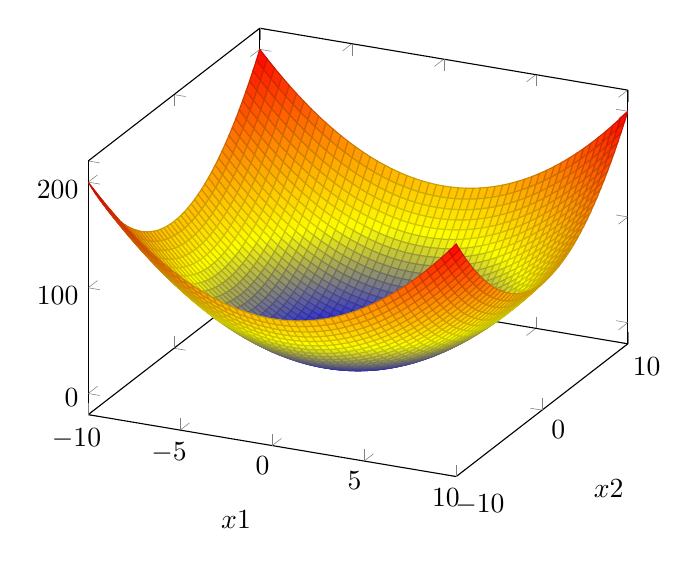
\begin{tikzpicture}
    \begin{axis}[
        xlabel=$x1$, ylabel=$x2$,
    ]
    \addplot3[surf, domain =-10:10, domain y=-10:10, unbounded coords=jump,
    samples=51]
        { x^2 + y^2 };
  \end{axis}
 \end{tikzpicture}
 
 \caption{DeJong's Function Graphic}
 \end{figure}


\subsubsection{Schwefel’s Function}
\begin{flalign*}
&f(x)  = \sum_{i=1}^n (-x_i sin(\sqrt{|x_i|})) \hspace{1cm} -500\le x_i \le 500&\\
&min(f(x))= -n\cdot418.9829&
\end{flalign*}

\begin{figure}[H]
  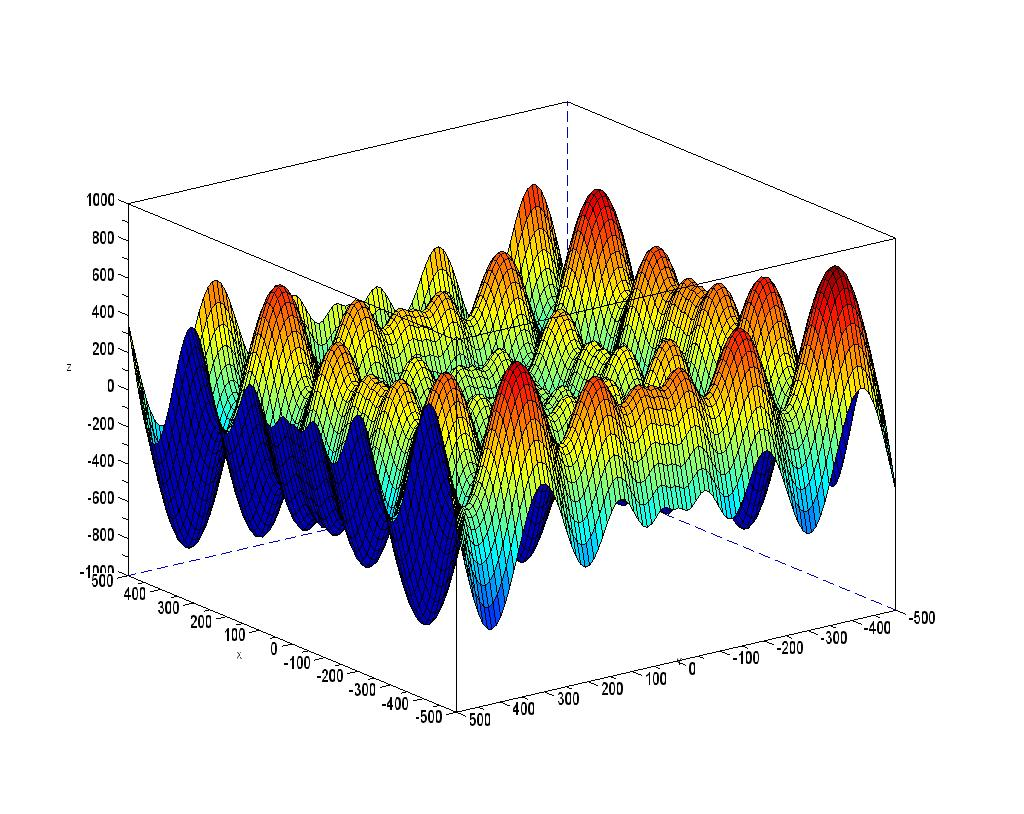
\includegraphics[width=0.6\textwidth]{schwefelsfunction.jpg}
  \caption{Schwefel's Function Graphic\cite{jamesmccaffrey}}
\end{figure}

\newpage
\subsubsection{Michalewicz’s Function}
\begin{flalign*}
&f(x) = - \sum_{i=1}^n sin(x_i) \cdot \left( sin\left( \frac{i\cdot x_i^2}{\pi} \right) \right)^{2 \cdot m} \hspace{1cm} m = 10, \hspace{0.3cm} 0\le x_i \le \pi&\\
&min(f(x))= -4.6876 \hspace{1cm} n=5&\\
&min(f(x))= -9.6601 \hspace{1cm} n=10&\\
&min(f(x))= -29.631 \hspace{1cm} n=30&
\end{flalign*}

\begin{figure}[H]
  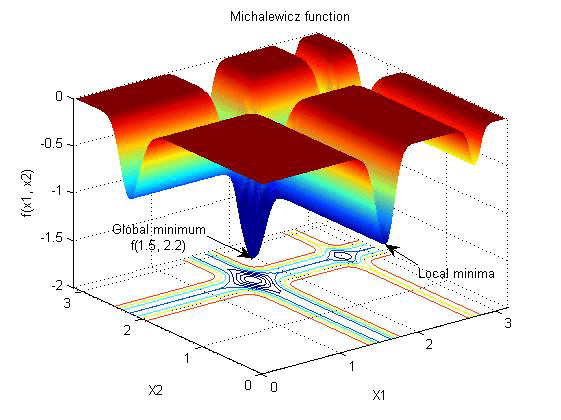
\includegraphics[width=0.6\textwidth]{michalewicz.png}
  \caption{Michalewicz's Function Graphic\cite{researchgate}}
\end{figure}


\subsubsection{Rastrigin’s Function}
\begin{flalign*}
&f(x) = 10 \cdot n + \sum_{i=1}^n (x_i^2 - 10 \cdot cos(2 \cdot \pi \cdot x_i)) \hspace{1cm} -5.12\le x_i \le 5.12&\\
&min(f(x))= 0&
\end{flalign*}

\begin{figure}[H]
  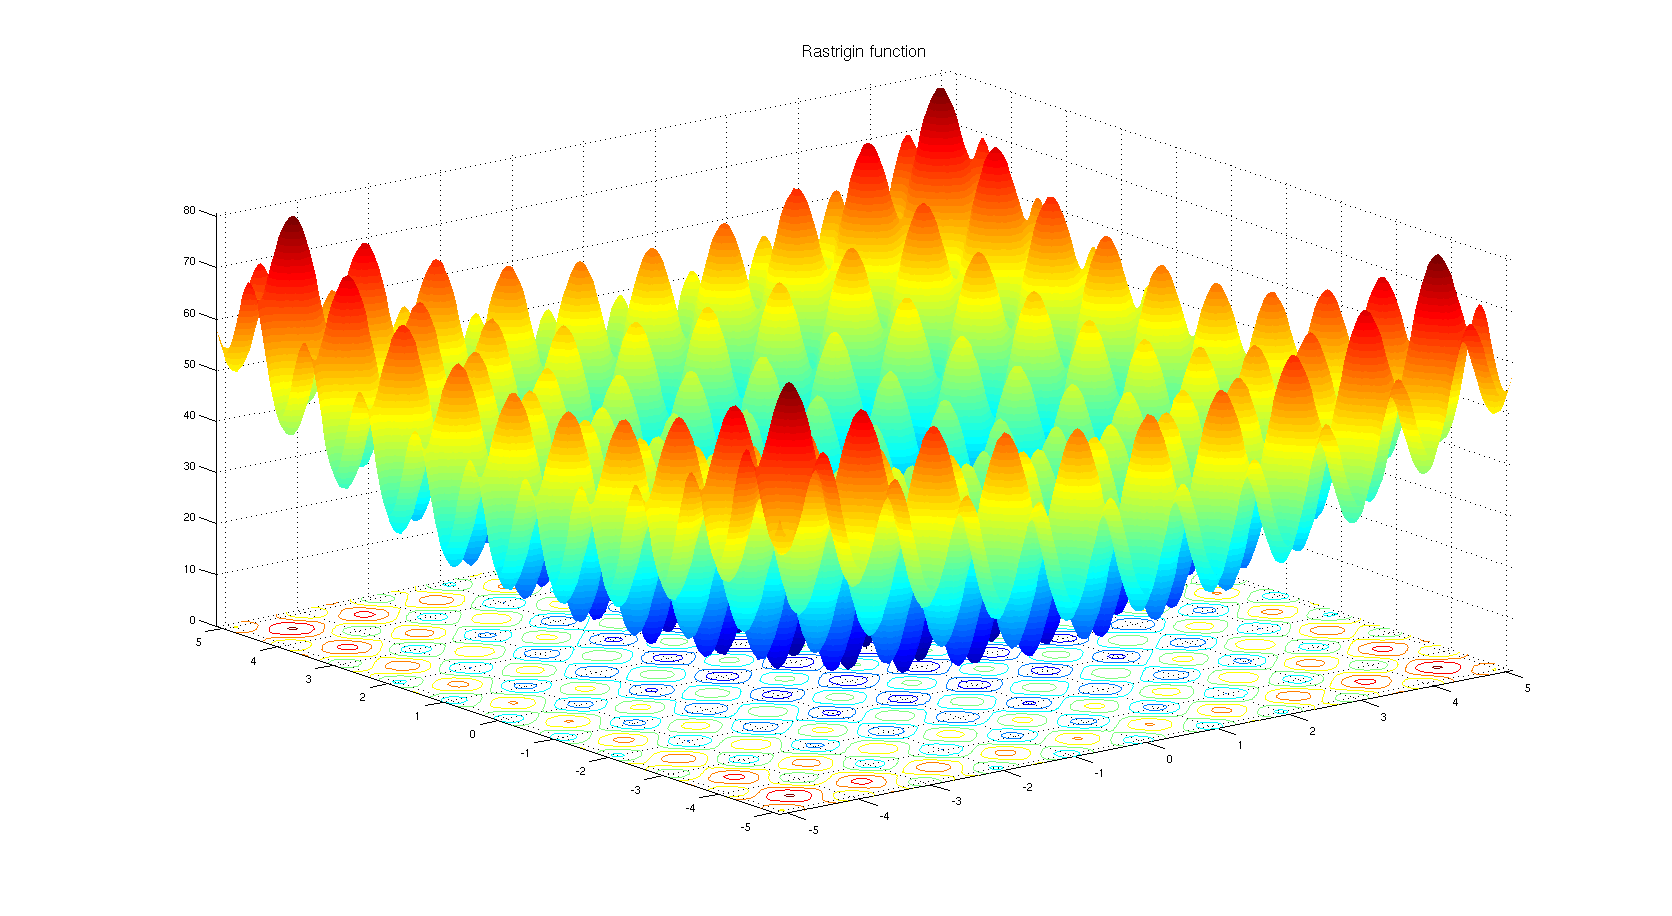
\includegraphics[width=0.6\textwidth]{Rastrigin.png}
  \caption{Rastrigin's Function Graphic\cite{wikiRastrigin}}
\end{figure}

\newpage
\subsection{Confidence Interval}
The confidence interval\cite{baltosser1996biostatistical} is defined as follows:
\begin{flalign*}
&CI=\overline{x}\pm z\frac{\sigma}{\sqrt{n}}&
\end{flalign*}

$\overline{x}$ is the sample \textbf{mean}

$z$ is the \textbf{confidence level}. 1.645 (90\%) is the convention standard

$\sigma$ is the sample \textbf{standard deviation}

$n$ is the sample \textbf{size}

\subsection{Describe Comparison Method}
Every function (De Jong 1 function, Schwefel's function, Rastrigin's function, Michalewicz's function) will be tested for 5, 10, and 30 dimensions.

\mSpace

The comparison is made between different versions of Genetic Algorithms(for selection is used Truncation Selection or Roulette Wheel Selection, and for crossover,  k-point crossover where $k \in {1, 2, 3, 4}$) on every benchmark function version.

The number of generations for every Ga is 1000, and the sample size for each test is 30.

\mSpace

The best Genetic Algorithm for each benchmark function is compared with the best strategy between Hill Climbing and Simulated Annealing for the same benchmark function \cite{HCSAME}.

The best strategy has the lowest mean and, if the mean is similar (the absolute value of the difference is lower than 0.1), is chosen the one with a lower margin of error.

\subsubsection{Hypotheses}

\begin{enumerate}
    \item RWS works better compared to Truncation Selection(TS), at least for wave functions
    
    \item Higher dimensions need more points in the k-point crossover

    \item The most noticeable difference between GAs and  Heuristic Algorithms (HA) is between functions of higher dimension, where the GA is the winner
    
    \item HAs work better for paraboloid types of functions due to their Hill Climbing Nature
\end{enumerate}

\newpage
\section{Genetic Algorithm Comparison}


\subsection{De Jong 1 Function}

\subsubsection{5 dimensions - Truncate Selection}
\CreateGraph{TS/dejong/5}{19}{0.000001}{0.1}

\subsubsection{5 dimensions - Roulette Wheel Selection}
\CreateGraph{RWS/dejong/5}{19}{0.000001}{0.1}


\subsubsection{10 dimensions - Truncate Selection}
\CreateGraph{TS/dejong/10}{19}{0.000001}{0.1}

\subsubsection{10 dimensions - Roulette Wheel Selection}
\CreateGraph{RWS/dejong/10}{19}{0.000001}{0.1}


\subsubsection{30 dimensions - Truncate Selection}
\CreateGraph{TS/dejong/30}{29}{0.00004}{0.02}

\subsubsection{30 dimensions - Roulette Wheel Selection}
\CreateGraph{RWS/dejong/30}{29}{0.000001}{0.1}


\newpage
\subsection{Schwefel’s Function}

\subsubsection{5 dimensions - Truncate Selection}
\CreateGraph{TS/schwefel/5}{199}{0.04}{0.02}

\subsubsection{5 dimensions - Roulette Wheel Selection}
\CreateGraph{RWS/schwefel/5}{199}{0.04}{0.02}


\subsubsection{10 dimensions - Truncate Selection}
\CreateGraph{TS/schwefel/10}{299}{1.5}{0.02}

\subsubsection{10 dimensions - Roulette Wheel Selection}
\CreateGraph{RWS/schwefel/10}{299}{0.6}{0.02}


\subsubsection{30 dimensions - Truncate Selection}
\CreateGraph{TS/schwefel/30}{399}{16}{0.02}

\subsubsection{30 dimensions - Roulette Wheel Selection}
\CreateGraph{RWS/schwefel/30}{399}{27}{0.02}


\newpage
\subsection{Michalewicz’s Function}

\subsubsection{5 dimensions - Truncate Selection}
\CreateGraph{TS/michalewicz/5}{74}{0.02}{0.02}

\subsubsection{5 dimensions - Roulette Wheel Selection}
\CreateGraph{RWS/michalewicz/5}{74}{0.03}{0.02}


\subsubsection{10 dimensions - Truncate Selection}
\CreateGraph{TS/michalewicz/10}{199}{0.06}{0.02}

\subsubsection{10 dimensions - Roulette Wheel Selection}
\CreateGraph{RWS/michalewicz/10}{199}{0.06}{0.02}


\subsubsection{30 dimensions - Truncate Selection}
\CreateGraph{TS/michalewicz/30}{399}{0.1}{0.02}

\subsubsection{30 dimensions - Roulette Wheel Selection}
\CreateGraph{RWS/michalewicz/30}{399}{0.15}{0.02}

\newpage
\subsection{Rastrigin’s Function}

\subsubsection{5 dimensions - Truncate Selection}
\CreateGraph{TS/rastrigin/5}{199}{0.3}{0.02}

\subsubsection{5 dimensions - Roulette Wheel Selection}
\CreateGraph{RWS/rastrigin/5}{199}{0.2}{0.02}

\subsubsection{10 dimensions - Truncate Selection}
\CreateGraph{TS/rastrigin/10}{199}{0.3}{0.02}

\subsubsection{10 dimensions - Roulette Wheel Selection}
\CreateGraph{RWS/rastrigin/10}{199}{0.3}{0.02}

\subsubsection{30 dimensions - Truncate Selection}
\CreateGraph{TS/rastrigin/30}{199}{1}{0.02}

\subsubsection{30 dimensions - Roulette Wheel Selection}
\CreateGraph{RWS/rastrigin/30}{199}{1}{0.02}

\newpage
\section{Heuristic Algorithms and Genetic Algorithms Comparison}
\subsection{De Jong 1 Function}
\begin{enumerate}
    \item \textit{RWS works better compared to Truncation Selection(TS)}
    
    \textbf{True} : Every algorithm finds a global minimum close to 0 but, for 30 dimensions, is clear that RWS is more consistent.
    
    \item \textit{Higher dimensions need more points in the k-point crossover}
    
    \textbf{Cannot Say} : The function is simple and the results are similar.

    \item \textit{The most noticeable difference between GAs and  Heuristic Algorithms (HA) is between functions of higher dimension, where the GA is the winner}
    
    \textbf{Cannot Say} : The function is simple and the results are similar.
    
\end{enumerate}

\subsection{Schwefel’s Function}
\begin{enumerate}
    \item \textit{RWS works better compared to Truncation Selection(TS)}
    
    \textbf{True} : In 5 dimensions, both strategies give similar results, but in 10 and 30, RWS has a lower average.
    
    \item \textit{Higher dimensions need more points in the k-point crossover}
    
    \textbf{False} : For this function, 3-point or 4-point crossover gives the best result for all dimensions.

    \item \textit{The most noticeable difference between GAs and  Heuristic Algorithms (HA) is between functions of higher dimension, where the GA is the winner}
    
    \textbf{True} : For 30 dimensions, The best GA (Roulette Wheel Selection with 3-Point Crossover with -12330.16227) has a much lower average value when compared to the best HA (Hill Climbing Best Improvement with -11378.970798).
    
\end{enumerate}

\subsection{Michalewicz’s Function}
\begin{enumerate}
    \item \textit{RWS works better compared to Truncation Selection(TS)}
    
    \textbf{True} : The difference is clear for 30 dimensions, where the best RWS (-27.43657) has a lower
minimum found compared to the best TS (-27.36678).
    
    \item \textit{Higher dimensions need more points in the k-point crossover}
    
    \textbf{False} : This function is the perfect counterexample, at least for dimensions lower or equal to 30. The tests show that 1-Point Crossover and 2-Points Crossover dominate in finding the best
global optima.

    \item \textit{The most noticeable difference between GAs and  Heuristic Algorithms (HA) is between functions of higher dimension, where the GA is the winner}
    
    \textbf{True} : For 30 dimensions, The best GA (Roulette Wheel Selection with 1-Point Crossover with
-27.43657) has a much lower average value when compared to the best HA (Hill Climbing Best
Improvement with -27.07615).
    
    
\end{enumerate}

\newpage
\subsection{Rastrigin’s Function}
\begin{enumerate}
    \item \textit{RWS works better compared to Truncation Selection(TS)}
    
    \textbf{True} : TS finds a lower average value for 5 and 10 dimensions, but 30, a much more complex function, RWS finds a lower average minimum.
    
    \item \textit{Higher dimensions need more points in the k-point crossover}
    
    \textbf{False} : The number of points in the k-point crossover is not directly proportional to the number of dimensions.

    \item \textit{The most noticeable difference between GAs and  Heuristic Algorithms (HA) is between functions of higher dimension, where the GA is the winner}
    
    \textbf{True} : For 30 dimensions, The best GA (Roulette Wheel Selection with 2-Point Crossover with 18.66132) has a much lower average value compared to the best HA (Hill Climbing Best Improvement with 28.633780).
    
\end{enumerate}

\section{Conclusion}
\begin{enumerate}
    \item \textit{RWS works better compared to Truncation Selection(TS), at least for wave functions}
    
    \textbf{True} : RWS finds a lower average value for most functions in 5 and 10 dimensions, but for 30 dimensions, RWS has a lower optimum for every benchmark function.
    
    \item \textit{Higher dimensions need more points in the k-point crossover}
    
    \textbf{False} : The number of points in the k-point crossover is not directly proportional to the number of dimensions.

    \item \textit{The most noticeable difference between GAs and  Heuristic Algorithms (HA) is between functions of higher dimension, where the GA is the winner}
    
    \textbf{True} : GAs find a lower optimum compared to any HA in any dimension.
    
    \item \textit{HAs work better for paraboloid types of functions due to their Hill Climbing Nature}
    
    \textbf{Cannot Say} : The function is simple and the results are similar.
    
\end{enumerate}

\bibliographystyle{alpha}
\bibliography{sample}

\end{document}